% !TEX encoding = UTF-8
% !TEX TS-program = pdflatex
% !TEX root = ../tesi.tex
% !TEX spellcheck = it-IT

%**************************************************************
\chapter{Descrizione dello stage}
\label{cap:descrizione-stage}
%**************************************************************

\intro{Breve introduzione al capitolo}\\
Questo capitolo tratterà l'organizzazione temporale del progetto, ovvero la sua divisione in attività e l'estensione temporale di ognuna. Il progetto è stato diviso in quattro fasi distinte, con diverse attività.


%**************************************************************
\section{Analisi preventiva dei rischi}

Durante la fase di analisi iniziale sono stati individuati alcuni possibili rischi a cui si potrà andare incontro.
Si è quindi proceduto a elaborare delle possibili soluzioni per far fronte a tali rischi.\\

\begin{risk}{Conflitti nell'implementazione parallela di \emph{User Stories}}
	\riskdescription{durante lo svolgimento di un progetto, ogni implementazione di una \emph{User Story} deve trovarsi su un \emph{branch} separato, derivato dal \emph{branch develop}. Può quindi accadere che, in determinati casi, l'esecuzione di ogni ticket e il suo assorbimento nel sistema non siano sequenziali, in quanto il Responsabile di progetto può non essere sempre presente. Quindi, nel caso in cui si realizzino più feature senza avere una \emph{pull request} alla fine di ognuna, il codice che poi dovrà essere inserito nel sistema darà quasi certamente conflitto nella fase di \emph{merge}}
	\risksolution{sollecitare il Responsabile di progetto all'analisi dei cambiamenti apportati ad ogni \emph{feature}, notificandolo periodicamente sullo stato di esecuzione del ticket, in modo che il Responsabile sia pronto all'esaminazione della \emph{User Story} implementata in modo più repentino}
	\label{risk:merge-conflict}
\end{risk}

\begin{risk}{Mancata competenza in strumenti e tecnologie aziendali}
	\riskdescription{al momento del mio inserimento in azienda, la mia competenza sull'applicazione di metodologie \emph{Agile} è stata pressoché nulla, così anche per quanto riguarda gli strumenti aziendali utilizzati in IKS e per determinate tecnologie da applicare durante il progetto. Questo fattore potrebbe portare ovviamente ad un rallentamento nel processo produttivo e, soprattutto, l'introduzione di errori}
	\risksolution{la prima attività che verrà svolta appena dopo l'inizio dello stage sarà appunto la formazione su tali tematiche. In particolare, come da Piano di Progetto, sono state stimate 40 ore di formazione per colmare le lacune da me possedute}
	\label{risk:tech-knowledge}
\end{risk}

\begin{risk}{Reperibilità del Responsabile di Progetto}
	\riskdescription{data la varietà di progetti che il Responsabile di Progetto a me assegnato deve seguire, può presentarsi la possibilità che questi non sia sempre reperibile in sede per un confronto diretto. Il rischio si applica anche a quelle giornate in cui il Responsabile è impegnato ad altri progetti aziendali per l'intera durata della giornata lavorativa.}
	\risksolution{la gestione delle attività tramite \emph{Kanban} serve proprio a mitigare questo tipo di rischi, in quanto uno sviluppatore può implementare più \emph{User Stories} senza dover consultare direttamente il Responsabile. Questo ovviamente se il Responsabile ha stilato un numero adeguato di \emph{User Stories} da implementare. Inoltre, l'utilizzo degli strumenti JIRA e STASH consente a due o più collaboratori di discutere il codice prodotto direttamente dall'interfaccia web, quindi anche in maniera telematica, ignorando il confronto diretto in sede}
	\label{risk:pm-availability}
\end{risk}

\begin{risk}{Cambiamento dei requisiti in corso d'opera}
	\riskdescription{data anche la natura mutevole di un ciclo di sviluppo software come la metodologia \emph{Agile}, è possibile che alcuni requisiti varino in corso d'opera, causando così una riorganizzazione di tempo e risorse non prevista}
	\risksolution{la presenza di uno strumento aziendale che fornisce lo stesso servizio consente una precisa individuazione dei requisiti ad inizio opera. Nel caso in cui vengano individuati requisiti aggiuntivi, il loro impatto sarà minimo e controllabile, aggiungendo le \emph{User Stories} corrispondenti nel \emph{backlog}}
\end{risk}

%**************************************************************
\section{Requisiti e obiettivi}
L'analisi dei Requisiti è stata svolta grazie alla suddivisione i storie intrinseca nella metodologia \emph{Agile}. Infatti, la stesura di una singola storia porta molte volte all'individuazione di uno o più requisiti, per la maggior parte funzionali.\\
La scelta delle storie da implementare è avvenuta tramite specificazione dei vari \emph{epic} noti all'inizio della pianificazione, successivamente spezzati in \emph{major} ed infine in \emph{User Stories} implementabili separatamente.

%**************************************************************
\section{Pianificazione}

\begin{figure}[H] 
    \centering 
    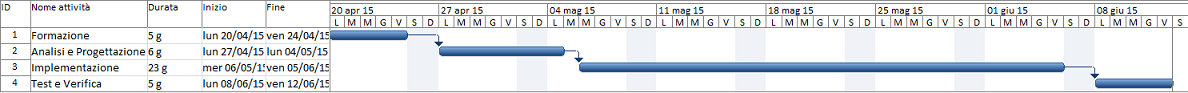
\includegraphics[width=1.1\columnwidth]{gantt_iniziale} 
    \caption{Diagramma Gantt della pianificazione iniziale}
\end{figure}

\subsection{Fase 1: Formazione (40 ore)}
Scopo: formazione sulle problematiche e tecnologie che si incontreranno durante lo stage.
In dettaglio:
\begin{itemize}
	\item AngularJS, \gls{rest} Angular, Jasmine, Istanbul;
	\item ambiente di sviluppo IKS (\gls{ide} per Javascript PhpStorm, Git);
	\item linee guida per lo sviluppo e concetti di programmazione sicura;
	\item verifica competenze acquisite.
\end{itemize}
Output (oggetto di verifica per il passaggio alla fase successiva):
\begin{itemize}
	\item predisposizione ambiente di sviluppo;
	\item realizzazione di una web application di esempio che utilizzi le tecnologie e gli approcci
indicati.
\end{itemize}

\subsection{Fase 2: Analisi e Progettazione (40 ore)}
Scopo: analisi delle specifiche funzionali, definizione del piano di test e progettazione tecnica
della soluzione da realizzare.\\
In dettaglio:
\begin{itemize}
	\item analisi specifiche funzionali;
	\item progettazione di dettaglio;
	\item documentazione.
\end{itemize}
Output (oggetto di verifica per il passaggio alla fase successiva):
\begin{itemize}
	\item documento di Specifica Tecnica;
	\item \emph{User Stories}.
\end{itemize}

\subsection{Fase 3: Implementazione (180 ore)}
Scopo: preparazione dell’ambiente di sviluppo e implementazione della soluzione.\\
In dettaglio:
\begin{itemize}
	\item implementazione tecnologica dei requisiti definiti in fase di analisi;
	\item documentazione.
\end{itemize}
\emph{Milestone} settimanali:
\begin{enumerate}
	\item realizzazione delle funzionalità di dialogo \gls{rest} con il \gls{back-end};
	\item creazione dell'interfaccia del profilo utente singolo;
	\item visione della gerarchia aziendale e dell'organizzazione per progetti dell'organico;
	\item gestione operazioni \gls{crud}\glsfirstoccur\  sui vari progetti aziendali e sui membri partecipanti.
\end{enumerate}
Output (oggetto di verifica per il passaggio alla fase successiva):
\begin{itemize}
	\item prodotto finale completo in tutte le sue parti;
	\item sorgenti commentati e pubblicati nel \emph{repository} dei sorgenti aziendale.
\end{itemize}

\subsection{Fase 4: Test e Verifica (40 ore)}
Scopo: Verifica funzionale, dei requisiti e stesura della documentazione.\\
In dettaglio:
\begin{itemize}
	\item analisi dei risultati;
	\item verifica funzionale;
	\item verifica dei requisiti di progetto;
	\item revisione e correzione di eventuali bug;
	\item documentazione;
	\item verifica finale.
\end{itemize}
Output (oggetto di verifica per la conclusione del progetto):
\begin{itemize}
	\item documento finale (conclusioni sull'attività di Stage svolta, con obiettivi raggiunti e
conoscenze acquisite);
	\item eliminazione di bug riscontrati e pubblicazione delle modifiche nel \emph{repository} dei sorgenti aziendale.
\end{itemize}

%************************************************************************